\documentclass[fr,license=none]{../../../eplsummary}

\usepackage{../../../eplcode}

\DeclareMathOperator{\pgcd}{PGCD}

\hypertitle[']{Informatique}{3}{FSAB}{1402}
{Beno\^it Legat\and Lucas Nyssens}
{Peter Van Roy}

\lstset{language={Oz},morekeywords={for,do}}

\newcommand{\st}{\mathrm{ST}}
\newcommand{\ce}{\mathrm{CE}}
\newcommand{\mozart}{Mozart}

\part{Programmation en \oz{}}
\section{Programmation déclarative}
La programmation déclarative est une programmation
dans laquelle les variables sont à affectation unique et
dans laquelle on écrit plutôt des fonctions récursives à la place
de boucles.

Le grand avantage de ce paradigme est qu'il reste déterministe,
même avec de la concurrence.

\section{Syntaxe et sémantique}
\subsection{Syntaxe et langage noyau}
La syntaxe, c'est la définition de ce qui peut être écrit.
Lors de la création d'un langage, on a envie que la syntaxe soit
stricte car c'est plus simple d'implémenter le langage ainsi mais
pour l'utilisateur, c'est plus rapide d'écrire avec une syntaxe
moins stricte.

Une manière de faire pour pallier ce problème est la création
d'un langage noyau dont la syntaxe est un sous-ensemble de celle
du langage.

La définition du langage est plus simple via ce langage noyau et
tous les éléments du langage peuvent être définis à partir du langage noyau.

\subsection{Sémantique}
La sémantique, c'est la description de ce que fait chaque élément
du langage.
Comme tout le langage peut être défini à partir du langage noyau,
il suffit de définir la sémantique du langage noyau et on définit toute
la sémantique.
Par contre, il faut traduire son programme en langage noyau
si on veut analyser sa sémantique.

En \oz{}, la sémantique se fait à l'aide d'une machine virtuelle.
Cette machine virtuelle est un tuple constitué de l'ensemble des
threads, de la mémoire à affectation unique $\sigma$ et de la mémoire
à affectation multiple $\mu$
\[ (\{\st_1, \ldots, \st_n\}, \sigma, \mu). \]
Chaque thread est représenté par une pile $\st_i$ consituée de couples
$(\verb|<s>|, \ce)$ où $\ce$ est l'environnement contextuel
de l'instruction \lstinline|<s>|
\[ \st_i = [(\verb|<s>|_1, \ce_1), \ldots, (\verb|<s>|_m, \ce_m)]. \]

La machine abstraite répète indéfiniment la même action jusqu'à ce
que toutes les piles soient vides ou qu'elles soient bloquées à cause du
dataflow (voir section~\ref{sec:dataflow}).
Durant cette action, elle choisit une pile.
Ce choix n'est pas arbitraire mais dépend de l'OS (Operating System) dans
lequel \mozart{} s'exécute.
Elle prend l'instruction au sommet de la pile $\verb|<s>|_1$ et l'exécute
avec comme environnement contextuel $\ce_1$.
Cette exécution dépend de l'instruction en question.
La sémantique des différentes instructions est donnée dans la suite de cette
synthèse.

Si on fait de la programmation déclarative, il n'y a plus de mémoire à
affectation multiple
\[ (\{\st_1, \ldots, \st_n\}, \sigma) \]
et si on ne fait pas de concurrence, il n'y a qu'une seule pile
\[ (\st, \sigma, \mu). \]
La programmation déclarative non concurrente est donc pourvue d'une machine abstraite
plus simple à utiliser
\[ (\st, \sigma). \]

\subsubsection{Cycle de vie d'un bloc mémoire}
\begin{figure}[htp]
\centering
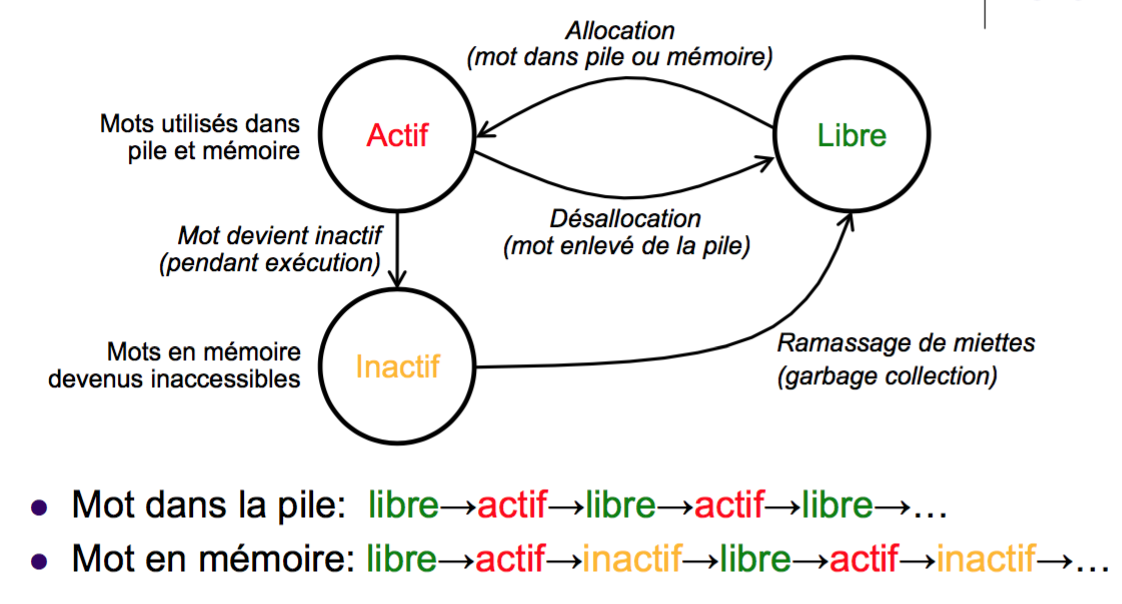
\includegraphics[scale = 0.4]{cycle.png}
\caption{Schéma du cycle de vie d’un bloc mémoire}
\label{cycle}
\end{figure} 

\subsubsection{Garbage collection}
Pour chaque variable en mémoire,
\oz{} se souvient du nombre d'identificateurs qui y sont liés.
Dès que ce nombre passe à zéro, \oz{} considère l'espace mémoire que
prenait la variable comme libre et on peut retirer la variable en mémoire
de la mémoire.

Par exemple, pour
\begin{lstlisting}
local B in
  local A in
    A = 0
  end
  B = 0
end
\end{lstlisting}
à la ligne 3, on a
\[ ([(3,\{\verb|A|\to a, \verb|B|\to b\}),
(5,\{\verb|B|\to b\})],\{a = 0, b\}) \]
et à la ligne 5, on a
\[ ([(5,\{\verb|B|\to b\})],\{b = 0\}) \]
où $a$ a été retiré de la mémoire car plus aucun identificateur ne
lui était associé.

\section{Instructions et expressions}
\label{sec:sv}
\oz{} fait une différence fondamentale entre expression et instruction.
D'ailleurs, en langage noyau, les seules ``lignes'' qu'il accepte sont les instructions.
En langage ``pas noyau'', par contre la dernière ``ligne''%
\footnote{Si la fonction termine par un block \lstinline|if ... elseif .. else ... end| ou \lstinline|case of ... [] ... end|, c'est la dernières ligne de chaque branchement.}
d'une fonction doit être une expression et non une instruction (cette expression est ce que la fonction renvoie).

Par exemple, si on essaie d'exécuter la ligne
\begin{lstlisting}
3
\end{lstlisting}
\oz{} nous dit
\begin{lstlisting}
%** expression at statement position
\end{lstlisting}
car il s'attend à ce que 3 soit une instruction.

Si on essaie d'appeler \lstinline{Foo} défini comme suit
\begin{lstlisting}
proc {Hello}
  {Browse 'Hello world'}
end
fun {Foo}
  {Hello}
end
\end{lstlisting}
\oz{} nous dit
\begin{lstlisting}
%** illegal arity in application
%**
%** Arity found:          1
%** Expected:             0
%** Application (names):  {Hello _}
%** Application (values): {<P/0> _<optimized>}
\end{lstlisting}
car comme \lstinline|Foo| est une fonction,
et que \lstinline|{Hello}| est la dernière ligne qu'il exécute,
il s'attend à ce que \lstinline|Hello| soit une fonction
et non une procédure.
En langage noyau, les fonctions sont des procédures avec un argument
en plus donc il veut donner un argument en plus à \lstinline|Hello|
mais \lstinline{Hello} ne prend pas d'argument d'où le
``\lstinline{illegal arity}''.

Comme vu plus haut,
\oz{} n'accepte que les instructions seulement en langage noyau.
Par exemple,
\begin{lstlisting}
A = 1
\end{lstlisting}
peut être utilisé comme expression et comme instruction.
En effet, du sucre syntaxique nous permet d'écrire
\begin{lstlisting}
B = A = 1
\end{lstlisting}
Seulement, en langage noyau, ça doit être écrit
\begin{lstlisting}
B = A
A = 1
\end{lstlisting}

\subsection{Composition séquentielle}
Dans le langage noyau, on parle toujours d'\emph{une} instruction
alors qu'en soit, parfois, on pourrait en mettre plusieurs.
Pour permettre cela, on rajoute la définition de composition séquentielle.
On dit qu'une instruction, ça peut être deux instructions.
Pour cela, on rajoute dans la syntaxe du langage noyau
\begin{lstlisting}
<s> ::= <s>_1 <s>_2
       | ...
\end{lstlisting}
où \lstinline|...| est constitué des autres syntaxes que peut prendre
une instruction.

Évidemment, 3 instructions par la composition séquentielle, c'est
aussi une seule instruction mais il faut effectuer deux compositions
séquentielles pour cela.

Cette définition est utile pour la sémantique.
Analysons la sémantique d'une composition séquentielle de l'instruction
\lstinline|<s>_1 <s>_2| d'environnement contextuel $\ce$.
La machine virtuelle ajoutera \lstinline|<s>_2| dans la pile
avec l'environnement contextuel $\ce$ puis elle ajoutera
\lstinline|<s>_1| avec l'environnement contextuel $\ce$.

Par exemple, la machine virtuelle transformera
\begin{lstlisting}
([(A = 1
   B = A + 1
   C = A + B, CE), ...], {a, ...})
\end{lstlisting}
en
\begin{lstlisting}
([(A = 1, CE),
  (B = A + 1
   C = A + B, CE), ...], {a, ...})
\end{lstlisting}
puis en
\begin{lstlisting}
([(B = A + 1
   C = A + B, CE), ...], {a=1, ...})
\end{lstlisting}
et ensuite en
\begin{lstlisting}
([(B = A + 1, CE),
  (C = A + B, CE), ...], {a=1, ...})
\end{lstlisting}

\subsection{L'instruction qui ne fait rien}
La syntaxe de \oz{} est plutôt stricte sur certains points.
Quand elle dit qu'elle veut une instruction, elle veut
soit une seule instruction, soit plusieurs car on peut considérer
que c'est une seule instruction avec la composition séquentielle mais
pas zéro instruction !

Par exemple
\begin{lstlisting}
if D \= 0 then
  F = N / D
else
end
\end{lstlisting}
n'est pas syntaxiquement valide.
Ça pose réellement problème car en langage noyau,
on ne peut pas omettre le \lstinline|else| (voir section~\ref{sec:if}).

\oz{} a donc une instruction qui ne fait rien, le \lstinline|skip|. Le code
\begin{lstlisting}
if D \= 0 then
  F = N / D
end
\end{lstlisting}
s'écrit donc
\begin{lstlisting}
local NotZero in
  NotZero = D \= 0
  if NotZero then
    F = N / D
  else
    skip
  end
end
\end{lstlisting}
en langage noyau.
La sémantique du \lstinline|skip| est assez simple.
On le retire tout simplement de la pile sans rien faire.

\section{Variables}
Les variables en \oz{} sont à affectation unique.
Quand elles sont à affectation multiple, on ne les appelle plus des variables
mais des cellules.

\subsection{Déclaration}
\label{sec:dec}
Pour créer une variable ou une cellule,
il faut d'abord créer un identificateur avec \lstinline|declare| ou un
\lstinline|local|.

\subsubsection{Le \keyword{} declare}
Il y a deux manière d'utiliser un \lstinline|declare|.
\begin{itemize}
  \item
    La première
    \begin{lstlisting}
declare <v>_1 <v>_2 ... <v>_n in
<s>
    \end{lstlisting}
    où les identificateurs \lstinline|<v>_i| sont créés
    avec une variable en mémoire associée.

  \item
    La seconde est un sucre syntaxique.
    \begin{lstlisting}
declare
<s>
    \end{lstlisting}
    \oz{} va lister tous les identificateurs utilisés dans \lstinline|<s>|
    qui ne sont pas dans l'environnement contextuel
    et va réécrire le code en langage noyau en mettant un \lstinline|in|
    avec ces identificateurs avant.
    Par exemple,
    \begin{lstlisting}
declare
A = 1
B = A + 1
    \end{lstlisting}
    va se réécrire
    \begin{lstlisting}
declare A B in
A = 1
B = A + 1
    \end{lstlisting}
    en langage noyau.
\end{itemize}
On peut remarquer que le \lstinline|declare| ne termine
pas par un \lstinline|end| mais par la fin du fichier (ou de la région
sélectionnée dans \mozart{}).
En effet, il est soit terminé par un autre \lstinline|declare| \footnote{Les identificateurs du premier \lstinline|declare| sont toujours accessibles après le second même si le premier est ``terminé''. C'est un \lstinline|declare|, pas un \lstinline|local| !}, soit par
une fin de fichier.

\subsubsection{Le \keyword{} local}
\lstinline|local| permet, tout comme le \lstinline|declare| de créer
des identificateurs mais lui peut être terminé par un \lstinline|end|.
Du coup, le \lstinline|declare| ne s'utilise souvent qu'une seule fois en
début de fichier alors que le \lstinline|local| s'utilise un peu partout.

Sa syntaxe dans le langage noyau est la suivante
\begin{lstlisting}
local <x> in <s> end
\end{lstlisting}
Pour définir sa sémantique, supposons que l'environnement du \lstinline|local|
était $\ce_1$.
Il ajoute \lstinline|(<s>, CE_2)| au dessus de sa pile d'instructions avec
$\ce_2 = \ce_1 + \{\verb|<x>| \to x\}$ où
$x$ est la variable en mémoire créée avec
\lstinline|<x>|.
On ajoute d'ailleurs $x$ à la mémoire, $\sigma' = \sigma \cup \{x\}$.

\paragraph{Raccourcis}
En sortant du langage noyau,
on peut utiliser un raccourci assez pratique pour éviter
d'écrire le mot local.
Après les \keywords{} \lstinline|proc|, \lstinline|fun| et
\lstinline|thread|, on peut ne pas écrire de \lstinline|local|.
% FIXME any other ?
Par exemple, dans
\begin{lstlisting}
proc {PrintAnswer}
  local
    fun {GetAnswer}
      42
    end
  in
    {Browse {GetAnswer}}
  end
end
\end{lstlisting}
la ligne 2 est optionnelle.

\subsection{Assignation}
Une variable peut avoir deux états (rien à voir avec les cellules)
\begin{itemize}
  \item Non assignée, c'est quand la variable en mémoire n'a pas encore
    de valeur, on peut alors lui assigner n'importe quelle valeur;
  \item Assignée, c'est quand la variable en mémoire a déjà une valeur.
    Dans ce cas, on peut lui assigner une valeur si et seulement si
    c'est la même valeur que celle qu'elle a déjà.
\end{itemize}

La syntaxe dans le langage noyau d'une assignation est la suivante
\begin{lstlisting}
<x> = <v>
\end{lstlisting}
mais le langage rend l'assignation symétrique.

Sémantiquement, la machine virtuelle assigne juste \lstinline|<v>| à
la variable en mémoire associée à \lstinline|<x>| dans
l'environnement contextuel.

Par exemple, dans
\begin{lstlisting}
local X Y in
  X = 1
  Y = 2
  local X in
    X = Y
  end
end
\end{lstlisting}
à la ligne 5, on a
\[ ([(X=Y, \{X\to x', Y\to y\})], \{x=1, x', y=2\}) \]
et la machine virtuelle transforme ça en
\[ ([], \{x=1, x'=2, y=2\}). \]

\section{Cellules}
Le concept d'objet est basé sur le fait qu'une fonction,
qu'on appelle alors \emph{méthode},
s'exécute avec un certain contexte.
Ce concept serait bien pauvre si ce contexte était constitué de constantes.

Tout comme en \java{}, en \oz{}, on sait créer des variables qui ne sont
pas constantes. On appelle ça des cellules.

\subsection{Création des cellules}
Pour créer des cellules,
on utilise la fonction \lstinline|NewCell|.
Par exemple,
\begin{lstlisting}
A = {NewCell 0}
\end{lstlisting}
Crée une nouvelle cellule avec comme valeur
\lstinline|0| et l'assigne à \lstinline|A|.
En langage noyau, ça donne
\begin{lstlisting}
local B in
  B = 0
  {NewCell B A}
end
\end{lstlisting}
Au niveau de la sémantique, il devrait déjà y avoir \lstinline|A->a|
dans $\ce{}$ et \lstinline|a| dans $\sigma$.
Après le \lstinline|local|, la composition séquentielle
et le \lstinline|B = 0|, on arrive à
(en considérant qu'on utilise pas de concurrence)
\[ ([(\verb|{NewCell B A}|, \{A\to a, B\to b, \ldots\}), \ldots],
\{a, b = 0, \ldots\}, \mu). \]
Après \lstinline|{NewCell B A}|, on aura
\[ \sigma = \{a = \xi, b = 0, \ldots\} \]
et
\[ \mu = \{a:b, \ldots\}. \]
$\xi$ est appelé le \emph{nom} de \lstinline|A|.

Il est vrai qu'on pourrait s'attendre à avoir $\xi:b$ dans
$\mu$ à la place de $a:b$.
Une discussion à ce sujet se trouve ici:
\begin{center}
  \url{http://www.forum-epl.be/viewtopic.php?t=11371}.
\end{center}

\subsection{Lecture d'une cellule}
L'instruction
\lstinline|A = B|
où \lstinline|B| est une cellule,
n'affecte pas à \lstinline|A| le contenu de \lstinline|B| mais leur donne
le même nom donc si on fait après \lstinline|A := 1|,
le contenu de \lstinline|B| sera changé aussi.

Pour lire le contenu d'une cellule, il faut utiliser \lstinline|@|.
Dans l'exemple précédent, l'expression \lstinline|@A| vaudrait \lstinline|b|,
c'est-à-dire 0.

\subsection{Écriture d'une cellule}
Pour écrire dans une cellule, il faut utiliser \lstinline|:=|.
Par exemple, à la ligne 4 de
\begin{lstlisting}
A = 0
B = 2
C = {NewCell A}
C := B
C := @C + 1
\end{lstlisting}
la machine virtuelle change la mémoire à affectation multiple
de \lstinline|{c:a,...}| à \lstinline|{c:b,...}|.

La ligne 5 s'écrirait en langage noyau en
\begin{lstlisting}
local D E in
  D = 1
  E = @C + D
  C := E
end
\end{lstlisting}
Pour la ligne 5, la machine virtuelle changerait la mémoire
à affectation multiple $\mu$ de
\lstinline|{c:b, ...}| à \lstinline|{c:e, ...}| où la mémoire
à affectation unique $\sigma$ vaudrait
\lstinline|{a=0, b=2, c=|$\xi$\lstinline|, d=1, e=3}|.


\section{Enregistrements, Tuples et Listes}
%      '|'
%      / \
%    42   nil
\subsection{Enregistrements}
Un enregistrement est constitué d'une étiquette, de champs et
d'un nom associé à chaque champ.
La syntaxe est la suivante
\begin{lstlisting}
<lit>(<f>_1:<x>_1 ... <f>_n:<x>_n)
\end{lstlisting}
où \lstinline|<lit>| est l'étiquette,
les \lstinline|<x>_i| sont les champs et
les \lstinline|<f>_i| sont les noms des champs.

Lors de la création d'un enregistrement,
on peut ne pas donner de nom à un champ.
\oz{} donnera $i$ comme nom au $i\ieme{}$ champ sans nom.
Si un autre champ de l'enregistrement possède déjà le nom $i$, \oz{} ne voudra pas fonctionner.

\subsection{Tuples}
Un tuple de $n$ champs est un enregistrement dont les noms des champs sont tous les entiers de
1 à $n$.

Par exemple,
\begin{lstlisting}
powers(1 2 4 8)
answers(42 21*2 '42' 'quarante-deux')
'#'(3 4 5)
3#4#5
\end{lstlisting}
sont des tuples.
\lstinline|#| donne une façon plus condensée d'écrire des tuples
dont l'étiquette est \lstinline|'#'|.
En effet, les lignes 3 et 4 sont équivalents.
Il est cependant important de constater que
\begin{lstlisting}
T = 5#6
4#T
\end{lstlisting}
ne produit pas \lstinline|'#'(4 5 6)| mais bien \lstinline|'#'(4 '#'(5 6))|.

\subsection{Listes}
Les listes ont une définition récursive.
C'est soit l'atome \lstinline|nil|,
soit un tuple d'étiquette \lstinline$'|'$ et de deux champ dont le
deuxième vaut une liste.

Par exemple,
\begin{lstlisting}
'|'(chien(nom:'Milou') '|'(chien(nom:'Idefix') nil))
\end{lstlisting}
est une liste.
On peut l'écrire de façon plus condensée en \oz{} de la manière suivante
\begin{lstlisting}
chien(nom:'Milou')|(chien(nom:'Idefix')|nil)
\end{lstlisting}
on peut même l'écrire
\begin{lstlisting}
[chien(nom:'Milou') chien(nom:'Idefix')]
\end{lstlisting}

\section{Structures conditionnelles}
%
%  /\  _____
% /??\/true
% \??/\_____
%  \/  false
Il y a deux types de structures conditionnelles en \oz{},
le \lstinline|if| et le \lstinline|case|.

\subsection{Structures conditionnelles par conditions}
\label{sec:if}
La syntaxe en langage noyau du \lstinline|if| est la
suivante
\begin{lstlisting}
if <x> then
  <s>_1
else
  <s>_2
end
\end{lstlisting}
où \lstinline|<x>| doit être de type \lstinline|boolean|.
D'un point de vue sémantique, supposons qu'on soit à
\[ ([(1-5,\ce),...], \sigma) \]
la machine abstraite va regarder la valeur de \lstinline|<x>|,
si elle vaut \lstinline|true|, alors, ça devient
\[ ([(2,\ce),...], \sigma) \]
sinon, ça devient
\[ ([(4,\ce),...], \sigma). \]

Au point de vue du langage,
on peut donner une expression comme condition,
on est pas obligé d'avoir un \lstinline|else|
et on peut même utiliser des \lstinline|elseif|.
Par exemple,
\begin{lstlisting}
if L == 'oz' orelse L == 'haskell' then
  Declarative = true
  ObjectOriented = true
elseif L == 'java' orelse L == 'C++' then
  Declarative = false
  ObjectOriented = true
elseif L == 'C' then
  Declarative = false
  ObjectOriented = false
end
\end{lstlisting}
est syntaxiquement correct.

\subsection{Manipulation de boolean}
Le type \lstinline|boolean| est constitué d'\lstinline|atom| qui valent
soit \lstinline|true|, soit \lstinline|false|.
Pour les manipuler, on a les 3 méthodes
\lstinline|Not|, \lstinline|And| et \lstinline|Or| ainsi que les deux
\keyword s \lstinline|orelse| et \lstinline|andthen|.
La méthode \lstinline|Not| est simple, elle inverse le boolean.
C'est l'équivalent de l'opérateur logique $\lnot$.

Les méthodes \lstinline|And| et \lstinline|Or| semblent faire
la même chose que \lstinline|orelse| et \lstinline|andthen| mais il y a
une différence importante.

Prenons comme exemple un fonction qui détermine
si \lstinline|B| est un diviseur de \lstinline|A|.
En utilisant \lstinline|andthen|, ça donne
\begin{lstlisting}
fun {DivisorOf B A}
  B \= 0 andthen (A mod B) == 0
end
\end{lstlisting}
On sait que si \lstinline|B| vaut 0,
\lstinline|A mod B| donne une erreur.
Seulement, avec \lstinline|andthen|,
\oz{} est malin et si \lstinline|B \= 0| vaut \lstinline|false|,
il se dit que quelque soit la valeur de \lstinline|(A mod B) == 0|,
l'expression totale vaudra \lstinline|false| et donc il ne l'évaluera
même pas.
En fait, en s'approchant du langage noyau, ça devient
\begin{lstlisting}
fun {DivisorOf B A}
  if B \= 0 then
    (A mod B) == 0
  else
    false
  end
end
\end{lstlisting}

Ce n'est pas le cas de la méthode \lstinline|And| qui est simplement
un appel de méthode.
Comme les deux expressions sont des arguments,
il faut les évaluer avant de les passer en argument.
\begin{lstlisting}
fun {DivisorOf B A}
  {And B \= 0 (A mod B) == 0}
end
\end{lstlisting}
devient donc, en s'approchant du langage noyau,
\begin{lstlisting}
fun {DivisorOf B A}
  local C D in
    C = B \= 0
    D = (A mod B) == 0
    {And C D}
  end
end
\end{lstlisting}
où \lstinline|(A mod B) == 0| est évaluée dans tous les cas.

Il y a une différence semblable entre l'expression
\lstinline|A orelse B| et l'expression \lstinline|{Or A B}|.
En effet, si \lstinline|A| vaut \lstinline|true|, dans le cas
du \lstinline|orelse|, \lstinline|B| n'est même pas évalué
alors que dans le cas du \lstinline|Or|, il est évalué.

\subsection{Structures conditionnelles par pattern matching}
Les \lstinline|if| sont bien pratiques pour comparer des nombres
mais quand il faut comparer des enregistrements, des tuples ou des listes,
c'est bien plus pratique de faire du pattern matching.

Pour faire du pattern matching,
il faut proposer un expression en partie construite et laisser
des variables pour les parties qu'on veut savoir
Par exemple, si on veut savoir le nom des personnes ayant comme prénom Jean,
il faut utiliser une clause avec \lstinline|personne(nom:Name prenom:Jean)|.

On rassemble les clauses dans un \lstinline|case| qui a la syntaxe suivante
\begin{lstlisting}
case <x>
of <clause>_1 then
  <s>_1
[] <clause>_2 then
  <s>_2
...
[] <clause>_n then
  <s>_n
else
  <s>_{n+1}
end
\end{lstlisting}
Du point de vue sémantique, soit $\ce$ l'environnement contextuel
du \lstinline|case|, la machine abstraite va trouver
la première clause qui correspond à \lstinline|<x>|.
\begin{itemize}
  \item Si elle n'en
    trouve pas, elle ajoute juste \lstinline|<s>_{n+1}| avec $\ce{}$ comme
    environnement contextuel;
  \item Sinon, elle crée une variable pour chaque variable
    de la clause qu'elle ne connaissait pas (disons $X$ et $Y$), ajoute l'instruction correspondante \lstinline|<s>_i| au sommet
    de la pile avec comme environnement contextuel
    $\ce + \{X\to x, Y\to y\}$ et associe à $x$ et $y$ (dans la mémoire) les valeurs correspondantes qu'elles avaient dans \lstinline|<x>|.
\end{itemize}

Prenons un exemple.
\begin{lstlisting}
case P
of personne(nom:Name prenom:'Jean') then
   {Browse Name}
[] personne(nom:'Dupont' prenom:Fname) then
   {Browse Fname}
[] chien(nom:'Milou') then
   {Browse 'Bonjour Milou, comment va Tintin ?'}
end
\end{lstlisting}
Ici, si \lstinline|P| vaut
\lstinline|personne(nom:'Dupont' prenom:'Jean')|.
Il n'y a que la première clause qui sera exécutée.
On passera de
\[ ([(1-8,\ce), \ldots], \sigma) \]
en
\[ ([(3,\ce+\{\verb|Name|\to\verb|name|\}), \ldots],
\sigma\cup\{\verb|name|=\verb|'Dupont'|\}). \]

La traduction en language noyau est la suivante
\begin{lstlisting}
case P
of personne(nom:Name prenom:'Jean') then
   {Browse Name}
else
   case P
   of personne(nom:'Dupont' prenom:Fname) then
       {Browse Fname}
   else
       case P
       of chien(nom:'Milou') then
           {Browse 'Bonjour Milou, comment va Tintin ?'}
       else
           raise missingElseClause end
       end
   end
end
\end{lstlisting}
On remarque que le \lstinline|else| est obligatoire en language noyau.

\section{Fonctions et procédures}
%   __               _ __  _ __ ___   ___
%  / _|_   _ _ __   | '_ \| '__/ _ \ / __|
% | |_| | | | '_ \  | |_) | | | (_) | (__
% |  _| |_| | | | | | .__/|_|  \___/ \___|
% |_|  \__,_|_| |_| |_|
\subsection{Procédures}
Une procédure en \oz{},
c'est une instruction
(qui peut être constituée de plusieurs instructions
par la composition séquentielle)
qui dépend de paramètres.

\subsubsection{Définition d'une procédure}
La syntaxe en langage noyau est la suivante
\begin{lstlisting}
proc {<x> <x>_1 <x>_2 ... <x>_n}
  <s>
end
\end{lstlisting}
mais ça peut aussi être écrit
\begin{lstlisting}
<x> = proc {$ <x>_1 <x>_2 ... <x>_n}
  <s>
end
\end{lstlisting}
mais cette écriture ne fait pas partie du langage noyau.

La sémantique est la même que pour l'assignation de variable sauf qu'ici,
la valeur est \lstinline|(proc {$ <x>_1 <x>_2 ... <x>_n} <s> end,CE)|
où $\ce$ est l'environnement duquel on ne conserve que les identificateurs
libres, c'est-à-dire les identificateurs qui sont déclarés avant la
procédure et qu'on utilise dans la procédure.

Il faut bien évidemment déclarer la variable \lstinline|<x>|
avec un \lstinline|declare| ou un \lstinline|local|
(voir section~\ref{sec:dec})
tout comme une variable à laquelle on assigne un entier.

Donc, par exemple, avec les lignes de 3 à 5 de
\begin{lstlisting}
local Answer in
  Answer = 42
  proc {GetAnswer X}
    X = Answer
  end
end
\end{lstlisting}
on passe de
\[
  ([(3-5, \{\verb|GetAnswer|\to\verb|getAnswer|,
  \verb|Answer|\to\verb|answer|,\ldots\}),\ldots],\sigma)
\]
où $\sigma = \{\verb|getAnswer|,\verb|answer|=42\ldots\}$
en $([\ldots],\sigma')$ où, dans $\sigma'$, \verb|getAnswer| devient
\[ \verb|getAnswer|=(\verb|proc {$ X} X = Answer end|,
  \{\verb|Answer|\to\verb|answer|\}). \]
On remarque que dans l'environnement contextuel de la cellule en mémoire,
on a gardé que \lstinline|Answer|, on a pas gardé les $\ldots$ car on utilisait
que \lstinline|Answer| ni \lstinline|getAnswer| car on ne faisait pas
de récursion ni même \lstinline|X| qui sera ajouté
lors de l'appel.

\subsubsection{Appel d'une procédure}
Pour appeler une procédure, la syntaxe est la suivante
\begin{lstlisting}
{<x> <x>_1 <x>_2 ... <x>_n}
\end{lstlisting}
où \lstinline|<x>| n'est pas spécialement le ``nom'' de la procédure.
Par exemple, on peut faire
\begin{lstlisting}
local B X in
  B = Answer
  {B X}
end
\end{lstlisting}
\lstinline|B| a la même valeur que
\lstinline|Answer| qui vaut la procédure,
c'est-à-dire que dans la mémoire,
on a
\[ \verb|b| = (\verb|proc {$ X} X = Answer end|,
\{\verb|Answer|\to\verb|answer|\})). \]
D'où la nécessité de garder les identificateurs libres dans la valeur
de la procédure car ici, \lstinline|B| n'est pas dans le
\lstinline|local Answer|.

Sémantiquement, ce qui va se passer c'est que la machine virtuelle
rajoutera sur la pile le contenu de la procédure avec son environnement
contextuel dont on ajoute les arguments.

Par exemple, dans l'exemple précédent, on passera de
\[ ([(\verb|{B X}|, \{\verb|B| \to \verb|b|, \verb|X| \to \verb|x|\},\ldots]
,\sigma) \]
à
\[ ([(\verb|X = Answer|,
\{\verb|X| = \verb|x|, \verb|Answer| = \verb|answer|\}, \ldots], \sigma). \]

\subsection{Fonctions}
Les fonctions ne sont pas définies dans le langage noyau.
Ce sont juste des procédures qui renvoient une valeur.
La syntaxe est la suivante
\begin{lstlisting}
fun {<x> <x>_1 <x>_2 ... <x>_n)
  <s> <v>
| <v>
end
\end{lstlisting}
C'est-à-dire que le corps de la fonction est soit constitué par une
instruction (ou plusieurs par la composition séquentielle)
suivie d'une expression, soit par une expression seule.
\footnote{Je n'aurais pas pu juste mettre \lstinline|<v>| en supposant
qu'il existe une composition
séquentielle \lstinline|<v> = <s> <v>_1| car c'est faux car en langage
noyau, il n'y a que des intructions, les expressions sont obligées de faire
partie d'une intruction (voir section~\ref{sec:sv}).}

Sa traduction en langage noyau est
\begin{lstlisting}
proc {<x> <x>_1 <x>_2 ... <x>_n <x>_{n+1})
  <s> <x>_{n+1} = <v>
| <x>_{n+1} = <v>
end
\end{lstlisting}

\subsection{Récursion}
\label{sec:rec}
Le principe de la récursion,
c'est qu'au lieu de calculer ce que doit faire la fonction,
on va établir une équation de récurrence avec un invariant et ça
va nous permettre de reléguer le travail à un appel récursif à la fonction
même qu'on écrit.
Bien sûr, il faut aussi un cas de base sinon la récursion sera
infinie.

Par exemple, imaginons qu'on veuille calculer le plus grand commun
diviseur ($\pgcd$) de deux nombres.
On vérifie sans mal que $\pgcd(a, b) = \pgcd(a-b, b)$.
Un corrolaire de la relation trouvée est
$\pgcd(a, b) = \pgcd(a \pmod{b}, b)$.
Durant l'exécution, faisons en sorte que $a > b$
sinon, on fait un coup pour rien donc utilisons
la relation de récurrence
$\pgcd(a, b) = \pgcd(b, a \pmod{b})$, en effet, n'oublions pas que
$a \pmod{b} < b$ par définition.
L'invariant, c'est $\pgcd(a,b)$.
Le cas de base, c'est $\pgcd(a, 0) = a$.
Ce cas tombe bien car $a \pmod{b}$ ne marche pas lorsque $b = 0$.
On a donc
\begin{lstlisting}
fun {PGCD A B}
  if B == 0 then
    A
  else
    {PGCD B A mod B}
  end
end
\end{lstlisting}

On peut calculer une complexité de $\bigoh(\log(\max(a, b)))$
ce qui est très efficace.

\subsubsection{Récursion terminale}
Il y a un problème avec les récursions,
du moins avec les langages classiques comme le \java{}.
À chaque appel, la pile augmente et à un moment, il n'y a plus
assez de mémoire.

Il y a une solution à ce problème en \oz{} qui requiert
un certain style de programmation qu'on appelle la récursion terminale.
Il faut qu'\emph{en langage noyau},
la dernière instruction à exécuter soit l'appel récursif.
Ainsi, il ne reste plus rien à exécuter pour chacune des fonctions
lorsqu'on fait l'appel récursive et la taille de la pile n'augmente pas.

Par chance, lors de la traduction en langage noyau automatique,
s'il y a moyen, \oz{} utilise toujours la récursion terminale.
Par exemple,
\begin{lstlisting}
fun {Sum N} % = 1 + 2 + ... + N
  if N == 0 then
    0
  else
    N + {Sum N-1}
  end
end
\end{lstlisting}
n'est pas récursif terminal car en langage noyau, ça donne
\begin{lstlisting}
proc {Sum N R}
  local Rec Z Eq in
    Z = 0
    Eq = N == Z
    if Eq then
      R = 0
    else
      Rec = {Sum N-1}
      R = N + Rec
    end
  end
end
\end{lstlisting}
par contre,
\begin{lstlisting}
fun {Sum N Acc}
  if N == 0 then
    Acc
  else
    {Sum N Acc + N}
  end
end
\end{lstlisting}
est récursif terminal ainsi que
\begin{lstlisting}
fun {ListNums N} % = [N N-1 ... 1]
  if N == 0 then
    nil
  else
    N|{ListNums N-1}
  end
end
\end{lstlisting}
parce que pour la créaction d'enregistrement,
les valeurs des champs \emph{peuvent être des variables pas encore assignées}.
Contrairement à l'opérateur $+$ où les deux opérandes doivent être connues.
Comme \oz{} est malin, il écrit alors le langage noyau comme suit
\begin{lstlisting}
fun {ListNums N R}
  local Z Eq in
    Z = 0
    Eq = N == 0
    if Eq then
      R = nil
    else
      local End in
        R = N|End
        End = {ListNums N-1}
      end
    end
  end
end
\end{lstlisting}

\subsection{Boucle for}
La boucle \lstinline|for|, c'est du pur sucre syntaxique.
Elle a deux formes.
La première,
\begin{lstlisting}
for <x> in <v> do <s> end
\end{lstlisting}
où \lstinline|<v>| doit être une liste.
La traduction en procédure est
\begin{lstlisting}
local
  proc {Loop L}
    case L of <x>|T then
      <s>
      {Loop T}
    else skip end
  end
in
  {Loop <v>}
end
\end{lstlisting}
La deuxième,
\begin{lstlisting}
for <x> in <int>_1...<int>_2 do <s> end
\end{lstlisting}
La traduction en procédure est
\begin{lstlisting}
local
  N = <int>_2
  proc {Loop I}
    if I =< N
      <s>
      {Loop I+1}
    else skip end
  end
in
  {Loop <int>_1}
end
\end{lstlisting}


\section{Concurrence}
\subsection{Concurrence}
Tout comme un ordinateur exécute plusieurs processus en même temps,
un programme peut avoir plusieurs threads.

En fait, le nombre de threads (tous processus confondus) qui peuvent
s'exécuter vraiment en même temps est égal au nombre de coeur mais
le système d'exploitation fait ce qu'on appelle du ``time sharing'',
c'est-à-dire qu'on l'impression que deux threads s'exécutent en même temps
mais en fait, on leur donne juste le processeur un temps très court puis
en le lui reprend et on le donne un temps très court à une autre.
Donc au final on sait exécuter beaucoup plus de threads en ``même temps''
qu'on a de coeur.

Pour lancer un thread en \oz{}, on utilise le \keyword{}
\lstinline|thread|. Sa syntaxe est la suivante
\begin{lstlisting}
  thread
    <s>
  end
\end{lstlisting}
Ce qui va se passer sémantiquement,
c'est qu'on va passer de
\[ ([(\verb|thread <s> end|,\ce),\ldots],\st_2, \ldots, \st_n,\sigma) \]
à
\[ ([\ldots],\st_2, \ldots, \st_n,[(\verb|<s>|,\ce)],\sigma). \]

\subsection{Dataflow}
\label{sec:dataflow}
On remarque que la mémoire est partagée entre tous les threads.
Si dans un thread on essaie d'évaluer une expression dont on ne connait pas
la valeur comme par exemple dans \lstinline|Y = X + 1| où \lstinline|X|
n'a pas encore de valeur mais \emph{pas} dans
\lstinline|answer(value:X)| ou \lstinline$42|X$ où on ne connait pas la
valeur de \lstinline|X|,
l'exécution se mettra en pause et attendra en esperant qu'un autre
thread lui assigne une valeur.
On appelle ça le ``variable dataflow''.

\subsection{Déterminisme}
Tout d'abord, insistons sur le fait que le mot ``déterminisme'' en
informatique n'est pas exactement le même qu'en philosophie où
on se demande des évènements sont purement aléatoire.
En informatique, on dit que c'est aléatoire quand ça dépend de facteurs
externes comme la température du processeur,
l'état du système d'exploitation,
etc, \ldots

On doit aussi se rendre compte que le temps donné à chaque thread
dépend du bon vouloir du système d'exploitation.
L'ordre d'exécution entre deux instructions dans deux threads différents
est rarement garanti.
Les seuls cas où c'est garanti, c'est quand on a par exemple
\begin{lstlisting}
thread Y in
  Y = X + 1
end
X = 41
\end{lstlisting}
où la ligne 4 s'exécutera toujours avant la ligne 2 si on imagine qu'aucune
autre ligne ne donne de valeur à \lstinline|X|.

Si on utilise des cellules,
notre programme devient \emph{non-déterministe}.
Par exemple, pour
\begin{lstlisting}
local Arch = {NewCell 0} in
  thread
    Arch = 32
  end
  thread
    Arch = 64
  end
  if Arch == 32 then
    {Browse ':('}
  elseif Arch == 64 then
    {Browse ':)'}
  else
    {Browse ':o'}
  end
end
\end{lstlisting}
on ne pourra jamais dire ce qu'affichera le programme.

Si on reste dans le modèle \emph{déclaratif},
l'exécution est néanmoins \emph{toujours déterministe}
car les variables ne peuvent pas changer de valeur donc au pire,
le programme attendra.

\section{Programmation orientée objet}
On peut faire de la programmation orientée objet
(abrégé POO en français et OOP en anglais) en \oz{} mais il
est pour cela \emph{nécessaire} de sortir du modèle déclaratif.
Il est donc impossible de faire de la POO concurrentielle déclarative.

La syntaxe d'une classe est la suivante
\begin{lstlisting}
class <x>
  attr <a>_1 <a>_2 ... <a>_n
  meth <m>_1 ... end
  meth <m>_m ... end
end
\end{lstlisting}
où on peut remarquer que tous les attributs doivent être déclaré
après un unique \keyword{} \lstinline|attr|.
Chaque attribut est une \emph{cellule} qui est créée automatiquement
mais sans être initialisée, c'est-à-dire que si on fait par exemple
\lstinline|@<a>_1 + 1| dès la création d'une cellule, ça va attendre
que la cellule ait une valeur.

La syntaxe de la définition d'une méthode est la suivante
\begin{lstlisting}
meth <m>(<x>_1 <x>_2 ... <x>_n)
  <s>
end
\end{lstlisting}

Pour en appeler une, la syntaxe est la suivante
\begin{lstlisting}
{<x> <m>(<x>_1 <x>_2 ... <x>_n)}
\end{lstlisting}
Que ce soit pour l'appel ou pour la définition d'une méthode,
s'il n'y a pas d'argument, les parenthèses sont facultatives.
Lors de l'implémentation d'une méthode,
pour appeler une méthode sur l'objet dans lequel on est,
il y a le \keyword{} \lstinline|self|.

Pour créer un objet, il faut utiliser la syntaxe suivante
\begin{lstlisting}
<x> = {New <x>_c <m>(<x>_1 <x>_2 ... <x>_n)}
\end{lstlisting}
où \lstinline|<x>_c| est la classe à instantier.

Les méthodes se comportent comme des procédures mais on peut aussi les
faire se comporter comme des fonctions.
Pour ce faire, il suffit de remplacer un \lstinline|<x>_i| lors de l'appel
et de la définition de la méthode en \lstinline|$|.
Bien évidemment, ils doivent être à la même place
(tous deux le \lstinline|i|\ieme{} argument).

Voici un exemple illustrant les concepts vu dans cette section
\begin{lstlisting}
declare
class Pair
  attr first second
  meth init(F S)
    first := F
    second := S
  end
  meth sort
     if @second < @first then
        {self swap}
     end
  end
  meth swap
     Tmp = @first
  in
     first := @second
     second := Tmp
  end
  meth getFirst($)
     @first
  end
  meth getSecond($)
     @second
  end
  meth multiply(A)
     first := @first * A
     second := @second * A
  end
end
X = {New Pair init(32 21)}
{X sort}
{X multiply(2)}
{Browse {X getFirst($)}}
\end{lstlisting}
Essayez de deviner ce que ce programme affiche.

\section{Type abstrait de données}
Celui-ci est une abstraction de données qui laisse les valeurs et les opérations séparées. On peut comparer ça à un distributeur automatique : les valeurs sont les pièces et les produits de la machine, les opérations sont les différents types de ditributeurs.

\begin{lstlisting}
local Wrap Unwrap in
    {NewWrapper Wrap Unwrap}
    
    fun{NewStack} {Wrap nil} end
    fun{Push W X} {Wrap X|{Unwrap W}} end
    fun{Pop W X} S={Unwrap W} in X=S.1 {Wrap S.2} end
    fun{IsEmpty W} {Unwrap W}==nil end
end
\end{lstlisting}

\section{Exceptions}
Comme en \java{}, en \oz{}, on sait lancer et traiter des exceptions.

\subsection{Traiter des exceptions}
Pour traiter des exception,
il faut utiliser le \keyword{} \lstinline|try| ainsi que
le \keyword{} \lstinline|catch|
\begin{lstlisting}
try <s>_1 catch <x> then <s>_2 end
\end{lstlisting}
Sémantiquement, on passe de
\[ ([(1,\ce),\ldots],\sigma) \]
à
\[ ([(\verb|<s>_1|,\ce),(\verb|catch <x> then <s>_2|,\ce),\ldots],\sigma). \]

\begin{figure}[htp]
\centering
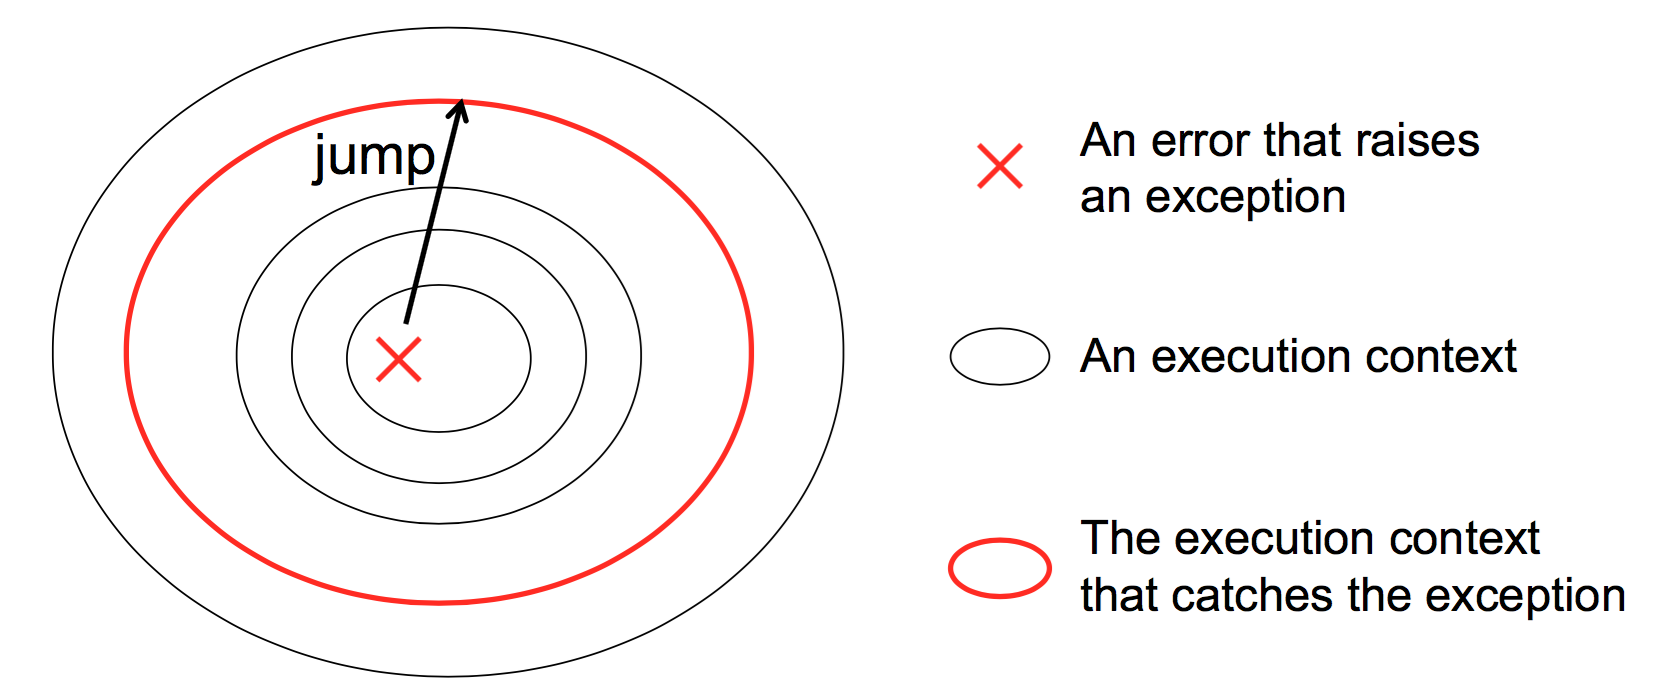
\includegraphics[width=.5\textwidth]{diagex.png}\hfill
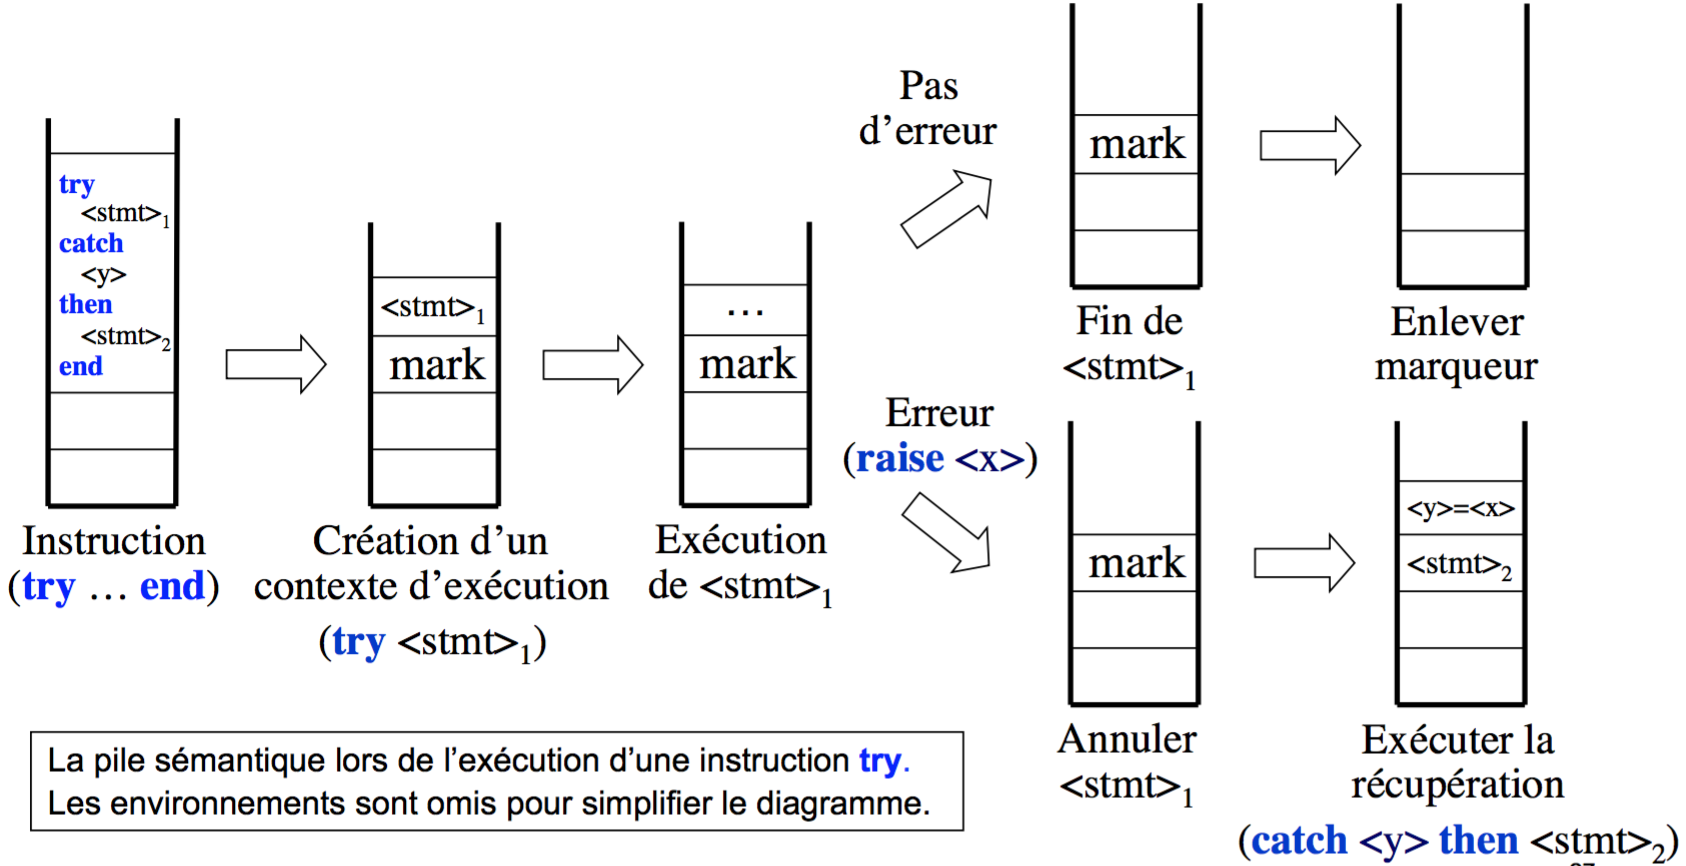
\includegraphics[width=.5\textwidth]{semex.png}\hfill
\caption{Diagrammes pour l'execution et la sémantique}
\label{GraphesRef}
\end{figure}

\subsection{Lancer des exceptions}
Pour traiter des exception,
il faut utiliser le \keyword{} \lstinline|raise|
\begin{lstlisting}
raise <x> end
\end{lstlisting}
Sémantiquement, la machine abstraite va dépiler chaque instruction
de la pile sans même les exécuter jusqu'à arriver à un \lstinline|catch|
qui correspond à \lstinline|<x>| au niveau du pattern matching.

Par exemple, on passe de
\[ ([(\verb|raise X end|,\ce_1),(\verb|R=S|,\ce_2),
(\verb|catch a(M) then skip end|,\ce_3), \]
\[ (\verb|catch b(M) then skip end|,\ce_4),\ldots],
\{x=\verb|b(v)|,v=\verb|'bla'|,\ldots\}) \]
en
\[ ([(\verb|skip|,\ce_4 + \{\verb|M|\to m\}),\ldots],
\{x=\verb|b(v)|,v=\verb|'bla'|,m=\verb|'bla'|,\ldots\}). \]

Voici un exemple illustratif sur les exceptions
\begin{lstlisting}
declare
fun {FunListInt List Fun}
   fun {FunListIntAux List Fun Acc}
      case List
      of H|T then
         if {IsInt H} then
            {FunListIntAux T Fun {Fun Acc H}}
         else
            raise nonIntFoundException(H) end
         end
      [] nil then
         Acc
      else
         raise invalidListException(List) end
      end
   end
in
   case List
   of nil then
      raise emptyListException() end
   [] H|T then
      {FunListIntAux T Fun H}
   else
      raise invalidListException(List) end
   end
end
fun {OpListInt List Op}
   Fun
   Default
in
   case Op
   of 'plus' then
      Fun = Number.'+'
      Default = 0
   [] 'times' then
      Fun = Number.'*'
      Default = 1
   [] 'max' then
      Fun = Max
      Default = none
   [] 'min' then
      Fun = Min
      Default = none
   else
      raise invalidOperandException(Op) end
   end
   try
      {FunListInt List Fun}
   catch emptyListException() then
      if Default \= none then
         Default
      else
         raise invalidListException() end
      end
   end
end
L = [32 42 troll 64]
try
   try
      try
         {Browse {OpListInt L 'plus'}}
      catch nonIntFoundException(M) then
         {Browse M}
      end
   catch invalidListException() then
      {Browse ':('}
   end
catch invalidOperandException(M) then
   {Browse M}
end
\end{lstlisting}
De la ligne 47 à 55,
il aurait été préférable de vérifier que la liste n'était pas vide
avant d'appeler \lstinline|FunListInt| car c'est considéré comme de
meilleure conception.
Cependant, dans le but d'illustrer les exceptions,
il a tout de même été choisi d'utiliser
l'exception \lstinline|invalidListException|.

\section{Complexité}
Pour évaluer l'efficacité tant temporelle que spatiale d'un programme,
on utilise la complexité.

\subsection{Complexité temporelle}
Le concept est simple.

Supposons qu'on ait obtenu une fonction $f(n_1, n_2, \ldots, n_m)$
qui décrit le nombre exact d'opérations à l'exécution en fonction
de paramètre $n_1, n_2, \ldots, n_m$ qu'on appelle la ``taille
du problème''.
Par la suite, prenons $m = 1$ et $n = n_1$ pour plus de simplicité.

C'est évidemment une supposition, en pratique,
on a jamais cette fonction.

On dit que la complexité temporelle est $\bigoh(g(n))$ si
$\exists C \in \mathbb{R}$ tel que $f(n) \leq C g(n)$.
C'est-à-dire que $g(n)$ est une approximation pessimiste de $f(n)$
à un facteur prêt.
On dit aussi que c'est la complexité du pire cas.
C'est très pratique car ça donne une bonne idée du temps
que l'exécution de dépassera jamais.

On dit aussi que la complexité temporelle est $\Omega(g(n))$ si
$\exists C \in \mathbb{R}$ tel que $C g(n) \leq f(n)$.
C'est-à-dire que $g(n)$ est une approximation optimiste de $g(n)$
à un facteur prêt.
On dit aussi que c'est la complexité dans le meilleur cas.
C'est moins pratique et moins utilisé que $\bigoh$.

On remarque que trouver un $g$ qui marche dans chaque cas
n'est pas bien compliqué. En effet dire qu'un algorithme est
$\Omega(0)$ est correct cependant, c'est d'une utilité assez limitée.
On essaie donc toujours de donner des approximation les plus proches
possible de $f$.

Parfois, on arrive à un $g$ identique pour $\bigoh$ et $\Omega$.
On dit alors que l'algorithme a une complexité $\Theta(g(n))$.

L'art réside souvent dans le choix d'une taille du problème qui
rendra le $g$ de $\bigoh$ et celui de $\Omega$ le plus proche possible
car, le plus on est précis, mieux c'est évidemment.

Par exemple, supposons qu'on veuille calculer un $\pgcd$
comme pour la section~\ref{sec:rec}.
L'algorithme dit ``brute-force'' car il cherche toute les possibilité
est le suivant
\begin{lstlisting}
fun {PGCD A B}
  fun {PGCDAux A B I}
    if A mod I == 0 andthen B mod I == 0 then
      I
    else
      {PGCDAux A B I-1}
    end
  end
  {PGCDAux A B {Min A B}}
end
\end{lstlisting}
Sa complexité est pas terrible, $\bigoh(\min(n,m))$ et $\Omega(1)$
où la taile du problème est $(n, m) = (a, b)$.
En effet, dans le pire cas, leur $\pgcd$ est 1 et dans le meilleur
cas, leur $\pgcd$ est $a$ ou $b$.

On a vu à la section~\ref{sec:rec} qu'il y avait une manière plus
efficace de calculer ce $\pgcd$.
\begin{lstlisting}
fun {PGCD A B}
  if B == 0
    A
  else
    {PGCD B A mod B}
  end
end
\end{lstlisting}
On peut se convaincre ici qu'en deux appels récursifs,
$a$ est au moins diminué de moitié.
En effet,
\begin{itemize}
  \item si $2b < a$, comme le $a$ de l'appel récursif est $b$, c'est
    vrai au premier appel;
  \item sinon, $a \pmod{b}$ est plus petit que la demi de $a$, au premier
    appel, il deviendra $b$ et au deuxième, il deviendra $a$.
\end{itemize}
En $\log_2(a)$ appels, on trouvera la solution.
Pour rester dans le pire cas, il faut prendre $\log_2(\max(a, b))$
donc la complexité est $\bigoh(\log_2(\max(n, m)))$ et $\Omega(1)$ où
la taille du problème est $(n,m) = (a, b)$.

\subsection{Complexité spatiale}
Pour la complexité spatiale, c'est exactement la même chose
sauf qu'au lieu de parler d'opération,
on parle de variable en mémoire qu'on ajoute à la mémoire.

\part{Définitions}
%    ________________________________________________
%   / ____        __ _       _ _   _                 \
%  / |  _ \  ___ / _(_)_ __ (_) |_(_) ___  _ __  ___  \
% |  | | | |/ _ \ |_| | '_ \| | __| |/ _ \| '_ \/ __|  |
% |  | |_| |  __/  _| | | | | | |_| | (_) | | | \__ \  |
%  \ |____/ \___|_| |_|_| |_|_|\__|_|\___/|_| |_|___/ /
%   \------------------------------------------------/
%     \               ,-----._
%   .  \         .  ,'        `-.__,------._
%  //   \      __\\'                        `-.
% ((    _____-'___))                           |
%  `:='/     (alf_/                            |
%  `.=|      |='                               |
%     |)   O |                                  \
%     |      |                               /\  \
%     |     /                          .    /  \  \
%     |    .-..__            ___   .--' \  |\   \  |
%    |o o  |     ``--.___.  /   `-'      \  \\   \ |
%     `--''        '  .' / /             |  | |   | \
%                  |  | / /              |  | |   mmm
%                  |  ||  |              | /| |
%                  ( .' \ \              || | |
%                  | |   \ \            // / /
%                  | |    \ \          || |_|
%                 /  |    |_/         /_|
%                /__/
\begin{description}
	
	\item[Dictionnaire]
	Tableau dynamique où les indices sont des constantes.
	
	\item[Loi de Moore]
	Le densité électronique des transistors dans une puce double tous les deux ans.
	
	\item[Ordre d'une procédure (ou fonction)]
	Une procédure est dite d'ordre N+1 si elle prend en argument une procédure d'ordre N maximum. Si elle ne contient pas de procédure on dit qu'elle est du premier ordre.
	
	\item[Problème NP-complet]
	(Non-déterministe Polynomial). En théorie de la complexité, un problème NP-complet (c'est-à-dire un problème complet pour la classe NP) est un problème de décision vérifiant les propriétés suivantes :
\begin{enumerate}

    \item Il est possible de vérifier un candidat solution efficacement en temps polynomial (la classe des problèmes vérifiant cette propriété est notée NP).
    \item Si on trouve un algorithme efficace pour résoudre le problème, on peut dériver un algorithme efficace pour tous les problèmes. Cela signifie que le problème est au moins aussi difficile que tous les autres problèmes de la classe NP (il est alors complet).
\end{enumerate}

	\item[Etat explicite]
	Séquence de valeurs calculées progressivement. Fonction qui évolue dans le temps, ayant une mémoire interne qui l’aide à faire son travail. Par exemple par l’utilisation de cellules.

  \item[Sucre syntaxique]
    Raccourci de notation qui n'a aucun effet sur l'exécution.

  \item[Identificateur]
    Nom introduit sur le clavier. Commence avec une majuscule.

  \item[Variable en mémoire]
    Partie de la mémoire dans le système, caché au programmeur.
    Représenté avec des minuscules.

  \item[Environnement]
    Fonction qui prend un identificateur et renvoie une variable.
    Il fait correspondre chaque identificateur
    à une variable en mémoire (et sa valeur).
    Un même identificateur peut correspondre
    à différentes variables en différents endroits du programme.

  \item[Portée lexicale]
    Partie d'un programme pour laquelle l'identificateur
    correspond à la même variable en mémoire.

  \item[Identificateur libre]
    Un identificateur libre d’une instruction est
    une occurrence d’un identificateur dans
    cette instruction qui n’est pas définie dans l’instruction.
    Pour une procédure,
    les identificateurs compris dans l'environnement contextuel,
    c'est-à-dire les identificateurs qui ne sont pas des paramètres
    de la procédure et qui ne sont pas déclarés dans la procédure.

  \item[Invariant]
    C'est une formule logique qui est vraie à chaque appel récursif.
    Il contient des informations globales
    (qui ne changent pas avec l'exécution ($n$))
    et locales (qui changent à chaque appel ($i$ et $a$)).
    Exemple:
    fonction qui calcule la $n\ieme{}$ puissance de $x$.
    Un invariant est $x^n = x^ia$.

  \item[Accumulateur]
    Se référer au principe des vases communiquant.
    Dans l'exemple précédent, l'accumulateur est $a$.

  \item[Récursion terminale]
    Une fonction est récursive terminale,
    si l'appel récursif est la dernière instruction à exécuter
    dans le corps de la fonction.
    Ainsi la taille de la pile d'instruction
    (cfr Sémantique) reste constante au fil des appels récursifs.

  \item[Spécification]
    Définition mathématique des entrées dont le programme a besoin et des résultats qu’il calcule.
    Exemple:
    définition de $x^n$. $x^0=1$; $x^{2n+1}=x\cdot x^{2n}$; $x^{2n} = (x^n)^2$.

  \item[Liste]
    Structure composée soit d'une liste vide (\lstinline|nil|),
    soit d'un élément suivi d'une autre liste.

  \item[Pattern matching]
    C'est la correspondance des formes.
    Il s'agit d'une succession de clauses.
    Une clause est exécutée,
    si la forme de l'élément dans l'instruction \lstinline|case| correspond à
    ce qui est compris dans la clause.
    La forme correspond si l'étiquette (label) et les arguments correspondent.
    Si c'est le cas,
    les identificateurs de la forme sont affectés aux parties correspondantes.
    Les clauses sont testées dans l'ordre textuel.
    La première à correspondre est exécutée et pas les autres.

  \item[Tuple]
    Structure composée d'une étiquette (label) et d'un nombre fini de champs.
    Les champs sont numérotés à partir de 1.

  \item[Enregistrement ou Record]
    Semblable à un Tuple, mais dont on peut définir le nom des champs.
    Les champs dont on n'a pas défini le nom sont numérotés à partir de 1.
    Deux champs ne peuvent pas avoir le même nom.

    Liste $\subset$ Tuple $\subset$ Record

  \item[Arbre]
    Il s'agit soit d'un nœud (Record) ou d'une feuille (\lstinline|leaf|).
    Chaque nœud comporte un ou plusieurs sous arbres (branches).
    Un arbre binaire est un arbre dont chaque nœud a deux branches.
    Un arbre est ordonné si, pour chaque nœud,
    la clé de leurs sous arbres de gauche (resp. droite)
    sont inférieures (supérieures) à la clé du nœud.

  \item[Sémantique]
    C'est ce que fait l'implémentation du langage de l'ordinateur.
    Il s'agit du modèle précis de l'exécution du langage de programmation.
    On l'utilise pour vérifier que le programme répond
    bien aux spécifications (souvent par preuve inductive).

  \item[Machine abstraite]
    Construction mathématique qui modélise l'exécution
    (ce sont les concepts utilisés pour effectuer
    la sémantique sur un programme).
    \begin{itemize}
      \item mémoire à affectation unique : variable et valeur (la valeur d'une variable ne change pas)
        $\sigma = \{ x=10, y=2, c=\xi\}$

      \item mémoire à affectation multiple : contenu des cellules
        $\mu = \{c:x\}$

      \item environnement:
        $E= \{ X\rightarrow x, Y \rightarrow y\}$

      \item instruction sémantique: instruction + son environnement
        $(<s>,E)$

      \item pile sémantique: pile d'instructions sémantiques
        $\st=[(<s_1>,E_1), \ldots, (<s_n>,E_n)]$

      \item exécution : séquence d'états d'exécution
        $(\st_1,\sigma_1)\rightarrow(\st_2,\sigma_2)\rightarrow
        \ldots \rightarrow(\st_n,\sigma_n)$
    \end{itemize}

  \item[Quelques règles de sémantique]

    Etat initial: $\st_0 =([(<s>,E=\emptyset)],\sigma_0=\emptyset)$

    A la fin: $ST_n =([],\sigma_n)$

    Environnement: adjonction $E_2 = E_1 \cup \{X\rightarrow x\}$
    sauf pour les appels de fonction: restriction à l'environnement contextuel.

    Composition séquentielle: $([(<s>,E)],\sigma)
    \rightarrow ([(<s_1>,E),(<s_2>,E)],\sigma)$

    Procédure en mémoire:
    $p = ($\lstinline|proc(|\$ \lstinline|X1 X2 \ldots) <s> end|$, \ce)$

  \item[Argument formel]
    Arguments dans la définition d'une procédure.
    Exemple:
    \lstinline|P = proc(|\$ \lstinline|X1 X2)|
    \lstinline|X1| et \lstinline|X2| sont des arguments formels.

  \item[Environnement contextuel]
    Environnement propre à une certaine procédure.
    Il fait le lien entre, uniquement,
    les identificateurs libres et leur variable en mémoire.

  \item[Valeur procédurale]
    Une valeur procédurale contient 2 choses: le code de la procédure
    et l'environment contextuel.

  \item[Cellule]
    C'est un conteneur avec une identité constante et un contenu variable.
    L'identité est le nom ou adresse de la cellule.
    Le contenu est associé à une variable qui est constante,
    mais la variable peut être remplacée par une autre.
    Il y a égalité entre deux cellules si ce sont les mêmes.

    Exemple : $\sigma = \{x=10, c=\xi\}$ et $\mu = \{c:x\}$
    Nous avons que $\xi$ est l'identité de \lstinline|C|, son contenu est $x$.

    En langage noyau, la construction d'une cellule est de la manière suivante:
    \lstinline|{NewCell I C}| ($\Leftrightarrow$ \lstinline|C = {NewCell I}|)

  \item[Modularité]
    On dit qu'un système (ou programme) est \emph{modulaire} si des mises
    à jour dans une partie du système n'obligent pas de changer le reste.
    L'état est bénéfique pour la modularité.

  \item[Encapsulation]
    Protéger l’intérieur d'une implémentation.

  \item[Abstraction]
    Définir une interface pour une
    interaction contrôlée avec l’intérieur, ce qui garantit
    un bon comportement. L’interface est un ensemble d’opérations qui peuvent être utilisées selon certaines règles. Il existe deux variétés principales d'abstraction de données : les objets et les type abstraits de données.

  \item[Polymorphisme]
    Une méthode est polymorphe si elle peut prendre
    des arguments différents et faire la même chose dans chacun des cas.
    Une telle méthode est reprise dans la définition d'une interface en java.

  \item[Héritage]
    Lorsqu'une classe \lstinline|A| hérite d'une classe \lstinline|B|,
    \lstinline|A| prend la définition de \lstinline|B|
    comme base (méthodes et attributs)
    et peut réécrire les méthodes de \lstinline|B| ou en ajouter.

  \item[Super-Classe]
    \lstinline|B| est une super-classe de \lstinline|A|
    si \lstinline|B| est dans la
    déclaration \lstinline|from| de \lstinline|A|
    ou est une super-classe d'une classe
    qui est dans la déclaration \lstinline|from| de \lstinline|A|.

  \item[Objet]
    Ensemble des procédures visibles (\lstinline|methode|) qui
    ont accès à un état caché dans une cellule (\lstinline|attribut|). Abstraction de donnée qui regroupe les valeurs et opérations en une seule entité.

  \item[Classe]
    Séparation entre définition d'objet et création. C’est une structure de données qui définit l’état interne d’un objet, son comportement et les classe dont il hérite. Une classe peut donner lieu à un nombre arbitraire d’instance. Dans Oz, une classe est un enregistrement qui contient un ensemble de noms d’attributs (sous forme d’une liste) et un ensemble de méthodes (sous forme d’un enregistrement).

  \item[Lien Dynamique]
    \lstinline|self| A utiliser par défaut,
    fait référence à l'objet qui appelle la méthode.

  \item[Lien Statique]
    Un appel
    \lstinline|SuperClasse,methode|
    dans une classe \lstinline|A|
    fait appel à la méthode décrite dans la classe \lstinline|SuperClasse|
    qui doit être une super-classe de \lstinline|A|.
    À utiliser uniquement pour la redéfinition d'une méthode
    déjà définie dans une super-classe.

  \item[Contexte d'exécution]
    Un contexte d’exécution est une partie de la pile sémantique
    qui commence avec un marqueur et qui va jusqu’au sommet
    de la pile.

  \item[Concurrence]
    Exécution de plusieurs activités au même temps.
    Elles peuvent communiquer (passer des informations de l'une à l'autre)
    et synchroniser (une activité attend une autre).

  \item[Exécution en Dataflow]
    Si on utilise une variable non initialisée,
    l'exécution attend qu'elle le soit.
    \lstinline|Browse| utilise un \lstinline|thread|,
    il actualise l'affichage quand un identificateur est lié.

  \item[Fil Thread]
    C'est une activité, une séquence d'instructions en exécution.
    Chaque fil est indépendant des autres,
    c'est-à-dire qu'il n'y a pas d'ordre entre eux.
    Deux fils communiquent s'ils partagent les mêmes variables.

  \item[Ordre total]
    Tous les états d'exécution d'un même fil font un ordre total.
    Dans un programme séquentiel (non concurrent), il existe un seul fil,
    l'ordre total décrit l'ordre entre chaque paire d'états.

  \item[Ordre partiel]
    Les états d'exécution du programme complet (s'il est concurrent)
    sont dans un ordre partiel.
    On ne connaît pas l'ordre d'exécution entre un état d'un fil
    et un autre d'un autre fil, ce pour chaque paire d'états du programme.

  \item[Non déterminisme]
    Ça apparait lorsqu'on utilise la concurrence avec les cellules.
    Absolument à éviter à cause de l'ordre partiel.
    Un programme concurrent est non déterministe
    si le résultat final n'est pas déterministe.

  \item[Flot]
    C'est une liste dont l'extrémité est une variable non liée.
    Ça sert comme canal de communication entre deux fils (agents).

  \item[Agent]
    Activité concurrente qui utilise un ou
    plusieurs canaux de communication (flots).

  \item[Producteur]
    Agent qui génère un flot de données.
    (Fonction utile: \lstinline|{Delay 1000}|
    met l'exécution en pause pendant une seconde).

  \item[Consommateur]
    Agent qui lit un flot de données. Généralement les affichent.
\end{description}


\annexe
\section{Installation et utilisation}
\subsection{Installation}
\subsubsection{Sous GNU/Linux}
Sous Debian/Ubuntu, voir le wiki communautaire d'Ubuntu
\begin{itemize}
  \item
    \url{https://help.ubuntu.com/community/Mozart}.
\end{itemize}

Pour les autres distribution, voir les liens suivant sur le site officiel
\begin{itemize}
  \item
    \url{http://www.mozart-oz.org/download/view.cgi?action=rpm&version=1.4.0};
  \item
    \url{http://www.mozart-oz.org/documentation/install/node2.html#chapter.rpm}.
\end{itemize}

\subsection{Utilisation}
\mozart{} est juste un plugin pour l'éditeur de texte GNU/Emacs.
Ce dernier est une éditeur de texte libre extrèmement puissant et complet.
Vous ne connaitrez sans doute jamais toutes ses fonctionnalités.

Pour pouvez par exemple essayer de taper \verb|M-x tetris| ou
\verb|M-x doctor| (\verb|M-x| signifie \verb|Alt + X|).

Néanmoins, pour développer en Oz, les fonctions utiles se trouvent
dans le sous-menu \emph{oz} de GNU/Emacs.

Voici les principales, données pour les régions mais elles sont pareilles
pour une ligne ou un buffer.
\begin{description}
  \item[Indent] Indente automatiquement la région sélectionnée.
  \item[Comment] Met la région sélectionnée en commentaire.
  \item[Core Syntax] Traduit la région sélectionnée en langage noyau.
  \item[Feed Region] Exécute la région sélectionnée.
  \item[Halt Oz] Interrompt l'exécution en cours.
\end{description}

\end{document}
